\section{Dossier de conception}

\subsection{Diagramme de classes}
\label{sec:diagramme-de-classes}

\begin{figure}[h!]
  \centerline{
  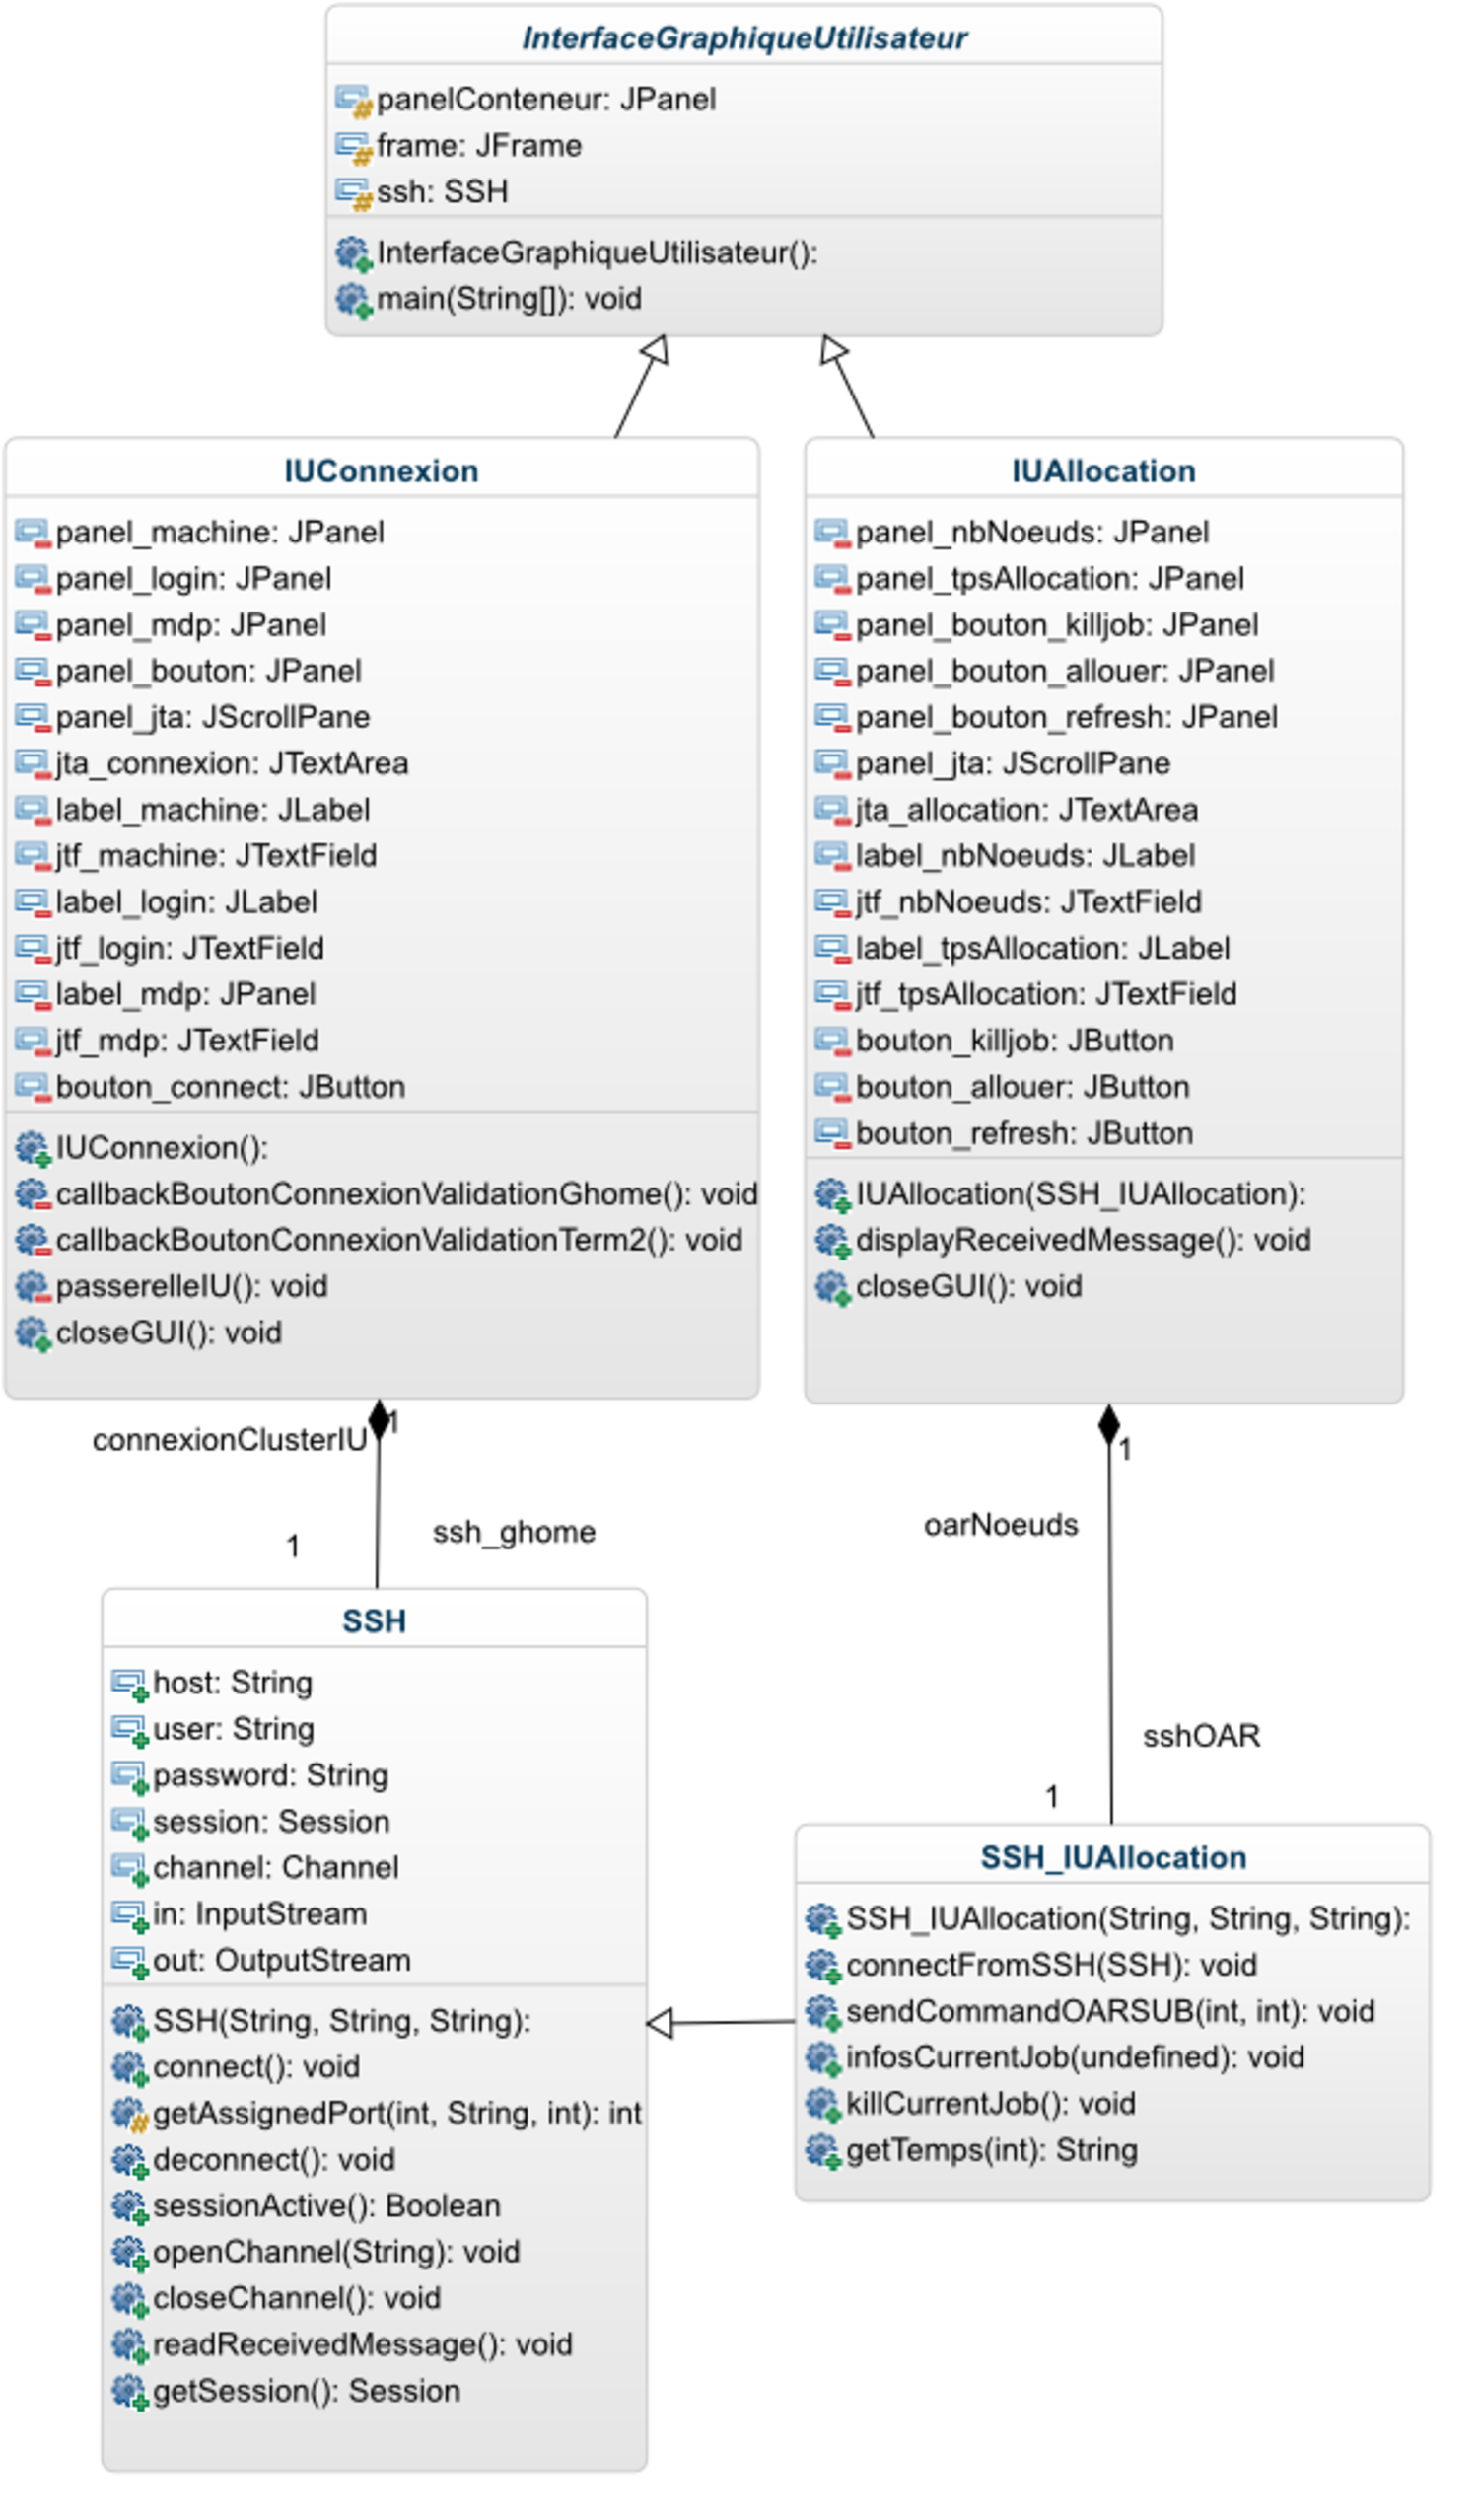
\includegraphics[width=18cm]{images/diagramme_classes.png}}
  \caption{Diagramme des classes}
  \label{fig:diag_classes}
\end{figure}

\subsection{Diagramme de séquence}
\label{sec:diagr-de-sequ}

\begin{figure}[h!]
  \centering
  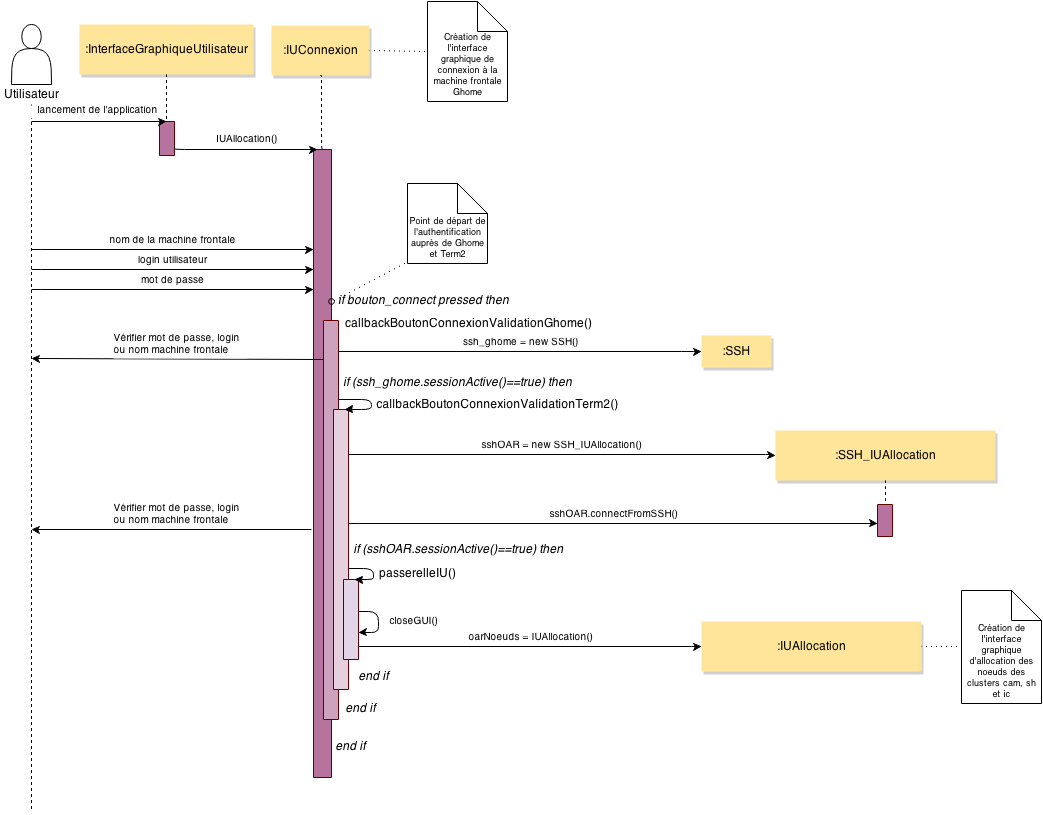
\includegraphics[width=16cm]{images/diagramme_sequence.png}
  \caption{Diagramme de séquence}
  \label{fig:diag_seq}
\end{figure}

\par La figure \ref{fig:diag_seq} donne le diagramme de séquence du scénario «Créer un job».  Tout d'abord, au lancement de l’application par l’utilisateur, l’IU de connexion s’affiche. L’utilisateur est en mesure de renseigner la machine sur laquelle il souhaite se logger, son nom d’utilisateur ainsi que son mot de passe. Lorsque les champs ont été convenablement remplis, l’appui sur le bouton de connexion lance le processus d’identification auprès des serveurs.
\par Une première session ssh est créée dans le serveur GHOME à partir de laquelle, sous condition qu’elle soit active, est créée une deuxième session ssh dans le serveur \texttt{TERM2}. S’il est impossible d’ouvrir une des deux sessions, alors un message d’erreur est renvoyé à l’utilisateur lui demandant de remplir à nouveau les champs. Dans le cas contraire, l’IU de connexion laisse sa place à l’IU d’allocation et le channel de type shell est créé afin d’envoyer les commandes au serveur.
\par L’utilisateur est désormais en mesure de remplir les champs «Nombre de nœuds» et «Temps d’allocation (en min)». L’appui sur le bouton allouer permet d’exécuter la commande ssh. Pour ce faire, plusieurs étapes sont nécessaires. Tout d’abord, les données rentrées par l’utilisateur doivent être traitées et mises sous forme d’une commande shell. La méthode \texttt{sendCommandOARSUB(nbNoeuds, tpsAllocation)} réalise cela en faisant appel à la méthode \texttt{getTemps(int)} afin de mettre sous forme xx:xx:xx heure:minutes:secondes) le temps d’allocation donné en minutes. La commande shell est créée et envoyée via le channel préalablement ouvert.
\par Une fois la commande shell envoyée, la méthode \texttt{readReceivedMessage()} se charge de rediriger vers l’utilisateur, à travers la \texttt{JTextArea} intégrée dans l’IU d’allocation, les données  renvoyées par le serveur. Ces données comprennent, conformément au cahier des charges la liste de nœuds alloués ainsi que les données décrivant l’état de création du job. 
\par Le rafraîchissement de la lecture des données en input du channel, donc provenant du serveur, est assuré par un objet de type Timer ayant pour but toutes les demi secondes de prendre la main afin de tester la présence de données en input. Les données retournées par le serveur semblent donc provenir en continu, sans que l'écoute ne monopolise le thread EDT.
\par Deux cas de figure se présentent à nous désormais concernant le scénario «Tuer le job». Soit le temps d’allocation est écoulé et dans ce cas le job est tué automatiquement par le serveur. Dans ce cas de figure le serveur se charge de reprendre les nœuds qu’il avait alloués. Donc aucune méthode java n’est nécessaire. 
\par Soit l’utilisateur a réalisé une mauvaise manipulation et n’a pas alloué le bon nombre de nœuds ou les a alloués pour une durée trop courte/trop longue (cf. scénario «Tuer le job»). Ici, l’utilisateur aura la possibilité de tuer le job afin d’en créer un nouveau à l’aide du bouton tuer qui appel la méthode \texttt{killCurrentJob()}. Cette méthode va tout simplement construire et envoyer la commande shell permettant de tuer le job courant en allant chercher au sein des variables d’environnement générées par OAR lors de la création du job son identifiant. Ceci évitera par exemple de tuer le job de quelqu’un d’autre.

\subsection{Fonctionnement de Swing}
\label{sec:fonct-de-swing}

AWT (Abstract Windowing Toolkit) est la bibliothèque graphique pour Java introduites dès ses premières versions. Depuis, d’autres API Graphiques ont vu le jour comme Swing, SWT et JFace qui permettent d’améliorer les performances (par exemple la rapidité de la gestion des évènements). Notre projet utilise la bibliothèque Swing, il nous semble par conséquent indispensable de comprendre son fonctionnement.
Swing est une des API Graphique les plus utilisées actuellement et très complexe. Elle est construite à partir de AWT. La majeure différence entre ces deux toolkit, outre leur API et leurs fonctionnalités, réside dans leur nature. En effet, AWT est dit heavyweight (ou lourd) tandis que Swing est dit lightweight (ou léger). Le premier terme désigne le fait que le toolkit est lié directement aux composants natifs nécessaires à l’affichage des applications graphiques alors que le deuxième prend complètement en charge la gestion des composants en les dessinant en pur Java.
Malgré ce degré d’abstraction vis-à-vis du OS, Swing nécessite AWT pour fonctionner. En outre, il utilise son système d’acheminement des évènements qui est la source des problèmes de performances. En effet, toute application Swing est composée de trois threads.
Le premier correspond au main application thread chargé de lancer la méthode main. Le deuxième est le toolkit thread qui a pour but de recevoir les évènements du OS (Ex: appui sur une touche du clavier, clic) et de les transmettre au event dispatching thread ou plus communément appelé EDT. Ce dernier thread est le plus important car il est chargé de répartir les évènements reçus vers les composants concernés et d’appeler les méthodes d’affichage.
Tâchons de mieux comprendre le trio de threads à travers un exemple. Supposons que nous ayons un JTextField et que l’on appuie sur la touche 7. Cet événement est reçu par le « toolkit thread » et traité par l’EDT qui met à jour l’affichage du JTextField en invoquant les méthodes nécessaires de l’IU.
Les applications développées avec la bibliothèque Swing sont réputées pour être lentes du fait que tous les évènements sont traités par un seul et même thread. On comprend très vite l’intérêt d’un traitement en parallèle avec l’intervention de plusieurs threads. Le fonctionnement de l’EDT est similaire à celui d’une file d’attente. Toutes les opérations s’enchaînant successivement, il y a risque de ralentissement de l’exécution d’une opération à cause d’une opération lente. Bien qu’il soit possible que les interfaces graphiques soient peu réactives avec le toolkit Swing, cette bibliothèque ne souffre en aucun cas de mauvaises performances car la compréhension de son fonctionnement (trio de threads) permet de réaliser des interfaces réactives à l’aide de plusieurs modèles de gestion des threads qui permettent de rendre l’API « thread safe » (i.e. que les méthodes peuvent être exécutées par plusieurs threads s’exécutant en même temps).

\par Nous avons été bloqués un bon moment à cause d'une mauvaise gestion du thread EDT. En effet, l'utilisation d'une boucle infinie pour vérifier le contenu du buffer \texttt{in} monopolisait le thread EDT, empêchant toute autre action, notamment la mise à jour du contenu des fenêtres graphiques, et également la gestion des autres événements. L'utilisation d'un Timer, qui execute à intervalles réguliers un morceau de code logé dans un objet \texttt{Runnable}, a permis de résoudre le problème, tout en gardant une réactivité équivalente.

%%% Local Variables: 
%%% mode: latex
%%% TeX-master: "CompteRendu"
%%% End: 
